\documentclass[10pt, letterpaper, twoside]{article}
\usepackage[utf8]{inputenc}
\usepackage{geometry}
\usepackage{hyperref}
\usepackage[english]{babel}
 \geometry{
 a4paper,
 total={170mm,257mm},
 left=20mm,
 top=20mm,
 }
\usepackage{graphicx}
\graphicspath{ {./images/} } 
\setcounter{section}{2}
\usepackage[font=small,labelfont=bf]{caption}
 
\title{Assignment 2 \\ Parallel Debugging and Performance Analysis}
\author{Smith Agarwal \\ Shyam Arumugaswamy \\ Siddhesh Kandarkar}
\date{November 27, 2018}
 
\begin{document}
 
\begin{titlepage}
\maketitle


\section{Understanding Parallel Programming Challenges}

\subsection{Task 1}

In this task, investigate and describe briefly in the report the following concepts:

\begin{enumerate}
\item \textbf{Race condition} 

Race condition is a situation in which multiple threads attempt to access and change the same data on shared memory space. It becomes a bug when events do not happen in the order the programmer intended. The term originates with the idea of two signals racing each other to influence the output first. In parallel computing, since the order in which threads access/write same data is not known to user but depends on the scheduler, the users must avoid race conditions when programming.  \\

\item \textbf{Deadlock} 

\url{[https://www.cse.msu.edu/~forsati/cse410s16/Lectures/Chapter%205.pdf]} \\
A deadlock is a situation in which two or more competing actions(here threads) are each waiting for the other to finish, and thus neither ever does.\\

\item \textbf{Heisenbug (observer’s effect) } 

\url{[https://en.wikipedia.org/wiki/Heisenbug]} \\
A heisenbug is a software bug that seems to disappear or alter its behavior when one attempts to study it. Heisenbugs occur because common attempts to debug a program, such as inserting output statements or running it in a debugger, usually modify the code, change the memory addresses of variables and the timing of its execution. \\

\item \textbf{Cache coherency and false sharing}

Data can be stored in multiple caches at any given time, especially in a parallel program as each thread may have its own cache. If data in one cache is updated then the other caches must be updated accordingly. When all caches are kept up to date, it is said that there is cache coherency. The updating of the caches is done cache line by cache line. Cache lines contain multiple data values. Sometimes it is possible that one thread changes just one value on a
cache line. If a different thread accesses a different value on that cache line, cache coherency will force the cache line to be updated even though this is not necessary. This is costly and unnecessary and is referred to as false sharing. \\

\item \textbf{Load imbalance} 

In a parallel program each thread or process has a load which is the quantity of work that it has to do. Load imbalance arises when one thread/process has significantly more to do than the others. This results in threads/processes idling while they wait for the thread with the largest load to complete its work. During this period the program is in effect running in serial and is thus not utilising the benefits of parallel programming. \\

\item \textbf{Amdahl’s law} 

Amdahl's law states that the performance speedup is limited by the inherently sequential part of the computation. If s is the execution time for inherently sequential computations, the speedup is limited by:  

\(speedup(p) =  \frac{time(1)}{time(p)} = \frac{time(1)}{ s\: +\: parallel\_time(p)} <= \frac{time(1)}{s} \) 

where s = execution time of sequential part of code and p = \# of processors 

Clearly as N approaches infinity, the speedup will asymptotically reach \( \frac{time(1)}{s} \). This is important for strong scaling applications. \\

\item \textbf{Parallelization overhead} 

A parallel program requires additional work that is not necessary for a serial program. This work is referred to as parallel overhead. It includes tasks such as starting and terminating threads and synchronising jobs. \\

\item \textbf{Floating-point arithmetic challenges} 

\begin{enumerate}

\item \textbf{Comparisons} 

Floating-point numbers are represented on computers with IEEE standards. This representation of a floating-point number is only an approximation, unlike integers (e.g. 1.5 could be 1.4999999999 on computers). Therefore when comparing two floating-point numbers, particularly when one of the values are result of computation, it is not advisable to compare them simply via in/equality operators (==, \textgreater , \textless ). Instead, it is safer to compare the subtracted value (difference between the two floats) to some very small value (e.g. 1e-15). \\

\item \textbf{Definition of a zero and signed zeros} 

\url{[https://en.wikipedia.org/wiki/Signed_zero]} \\
In floating point numbers zero is signed so there is a positive zero and a negative zero. In most run-time environments, positive zero is usually printed as "0" and the negative zero as "-0". This can cause a problem in some instances. 1/(-0) returns negative infinity, while 1/+0 returns positive infinity. \\

\item \textbf{Cancellation or loss of significance} 

\url{[https://en.wikipedia.org/wiki/Loss_of_significance]} \\
Loss of significance occurs when an operation on two numbers increases relative error substantially more than it increases absolute error, for example in subtracting two nearly equal numbers (known as catastrophic cancellation). The following is an example of such operation, and four significant digits are lost for this example. 

$x = 1.23467 . 10^0 $ 

$y = 1.23456 . 10^0 $  

$x - y = 0.00011 . 10^0 = 1.1 . 10^{-4} $ \\

\item \textbf{Amplification and error propagation} 

\url{[https://en.wikipedia.org/wiki/Round-off_error]} \\
Amplification errors occur when a number cannot be represented exactly in floating point arithmetic. Then, if a series of calculations is performed on an unexactly represented number, this error is amplified. \\

\end{enumerate} 

\end{enumerate} 

\subsubsection{Questions}

\begin{enumerate}
	\item\textbf{Which of the concepts affect performance but not correctness?} 
	
	Parallel overhead will of course affect performance as it is extra work for the program to do. It does not however directly affect the result of the program and therefore does not affect correctness. Load imbalance can affect performance although it will not affect correctness. The worse the imbalance, the worse the effect on the performance. In the worst case the code will in effect run in serial (with the parallel overhead in addition to the steps that would have
occurred if the program had been run entirely in serial). If cache coherency is assured then the correctness of the program will not be affected, however the process of keeping the cache up to date can be costly, especially in the case of false sharing. This therefore affects performance. Deadlock could also be considered to affect
performance. This is arguable since deadlock just stops the program, but to solve deadlocks blocking-operations and/or synchronisation are often required which causes overhead. \\
	
	\item\textbf{Which of the concepts affect the correctness of the application?} 
	
	If the cache is not coherent then read values may be incorrect, This will obviously lead to incorrect results. Any computations involving floating-point operations are also clearly subject to incorrect results. Race conditions may also lead to incorrect results if read and write operations are conducted in an unintended fashion/order. Finally, although not always applicable, Heisenbug can also be considered since the program may not work as intended when some code lines (e.g. cout) for debugging purposes are added/removed.  
	
\begin{enumerate}
\item \textbf{Of these, which are exclusive to parallel programming?} 

Problems due to a lack of cache coherency are exclusive to parallel programming as a serial program has no reason to store the same variable in multiple caches. Another concept exclusive to parallel programming is race condition, since it occurs only for multi-
threaded computing paradigm. 

\item \textbf{Of these, which are not exclusive to parallel programming?} 

Floating-point arithmetics are obviously not exclusive to parallel programming, and are common problems in any programming paradigm.
Heisenbug (if considered to affect the correctness of the program) is also not exclusive to parallel programming.\\
\end{enumerate}

\item\textbf{Which of them can occur in OpenMP applications?}
 
False sharing can occur in OpenMP as it is a shared memory system and therefore all threads should have access to the same up-to-date information. Load imbalance can occur in OpenMP however, there are multiple load balancing methods (static, dynamic, guided, auto, runtime) which which therefore allow an optimal configuration to be used to try and reduce this. As with all parallel programs, OpenMP has parallel overhead. Both race condition and deadlock can occur in
multi-threaded computing paradigm on shared memory systems, hence OpenMP.	\\

\item\textbf{Which of them can occur in MPI applications?} 

As with all parallel programs, MPI has parallel overhead. MPI can also have load imbalance problems. Although it is designed in such a way that all threads carry out the same tasks simultaneously, if loops can result in different loads for different processes and thus
load imbalance. Deadlock can occur in MPI applications too, for instance by using MPI\_Send and MPI\_Recv commands separately (instead of MPI\_sendrecv). MPI\_Send and MPI\_Recv are blocking operations. MPI\_Send blocks until the data in sending buffer is received by the receiving buffer, and MPI\_Recv blocks until the data is received in the receiving buffer. Similar to thread-wise deadlock explained above, deadlocks can occur in MPI applications if such blocking forms a loop/symmetry. \\

\item\textbf{Is cache coherency necessary on MPI applications with a single process and a single thread per rank? Explain.} 

Cache coherency is not necessary when there is a single process and a single thread as there is no parallelism and thus no reason for the same data to be stored in multiple places. The rank identifies the process within a MPI communication group. When there is only one process, there is no need for communication, however it is still possible to create multiple groups. This arises when a program
designed to be run with multiple processes is run with only one process. Thus it is possible to create one thread per rank and therefore use multiple threads. Threads use a shared memory model which means that all threads should have access to the same data, thus in this case cache coherency is necessary. \\

\item\textbf{Is Amdahl’s law applicable to strong scaling applications? Explain.} 

Yes, it is applicable to strong scaling applications. A strong scaling application is not able to scale linearly for large N due to
inherently serial code in the application as well as communication overhead. When the amount of processing elements are increased for a strong scaling application, the inherently serial part of the code will not benefit and communication between processing units increases, which will both prevent linear scaling. Therefore, a large scaling application will scale asymptotically towards \( \frac{time(1)}{s} \) as N processing elements increases. As stated above, \( \frac{time(1)}{s} \) is also the upper limit in Amdahl's Law. \\

\item\textbf{Is Amdahl’s law applicable to weak scaling applications? Explain.} 

Amdahl's law is applicable to fixed workload applications. However, weak scaling applications do not respect this assumption and therefore, Amdahl's law is not applicable to weak scaling applications. Linear scalability can be achieved with weak scaling applications due to the fixed workload assumption being relaxed. Since the assumption that workload is relaxed and workload varies linearly with N, we are able to have a linear speedup, although the slope of the speedup will most likely be less than 1. However, if workload were to remain constant, then Amdahl's law would be apparent in weak scaling applications, as processing units increase. \\

\item\textbf{Which of these limit the scalability of applications?} 
 
As previously mentioned, parallel overhead affects the performance of the program. The more threads are used, the larger the overhead becomes. At some point this may begin to be one of the slowest parts of the program. It therefore limits the scalability. Equally
any problems which lead to more overhead such as false sharing, or the synchronisation or mutexes required to avoid race conditions or deadlocks, also limit the scalability of applications. \\

\end{enumerate}

\setcounter{section}{4}
\section { TotalView GUI}

TotalView is a parallel debugger offered by Rogue Wave Software. It is supported in several large computer centers in the world. With TotalView , developers can inspect source code, control threads and processes, inspect memory and state, etc . It supports C, C ++ and Fortran applications, as well as multiple threads with OpenMP and multiple processes with MPI. \\

\subsection {Task 2}

The following are some of the aspects of TotalView's GUI

\begin{enumerate}
\item \textbf{Session Manager}:

Very first pane at user sees when invoking totalview . It allows the user to launch a new program (serial or parallel), attach to a running program, load a core file, save a debug session for later, or
load a previously saved debug session. \\

\item \textbf{Root Window}:

Appears when TotalView is started. Provides an overview of all processes and threads the TotalView assigned ID, MPI rank, status, and letter description / name for each. Allows sorting on each
column of information that appears. Provides the ability to expand / collapse information under the hostname column. The "Configure" button allows selection of which information is displayed. \\


\item \textbf{Process Window}:

Provides information on debugging / testing process. By default, a single process window want display. For multi-process / multi-threaded programs, however, every process and every thread may have
its own Process Window if desired. Contains the following 4 panes. 

\begin{enumerate}
\item \textbf{Stack Trace Pane}:

Shows the call stack of routines the current executable is running. Selection of any routine shown in the call stack will automatically update the Process Window with its information. \\


\item \textbf{Stack Frame Pane}:

Displays the local variables, registers and function parameters for the selected executable. Register abbreviations and meanings are architecture specific. \\


\item \textbf{Source Pane}:

Displays source code for the currently selected program or function. Shows program counter, line numbers and any associated action points. Only the lines with a "box" on their line numbers are eligible for debugging. \\

\item \textbf{Action Points, Processes, Threads Pane}:

A multi-function pane. By default, it shows any action points
that have been set. Action points are either a breakpoint, a barrier point, an eval point, or a watchpoint. The threads tab may also be selected to show associated threads. \\
\end{enumerate}

\item \textbf{Variable Window}:

Appears when user dives on a variable or selects a menu item to view variable information. Displays detailed information about selected program variables. Permits editing, diving, filtering and sorting of variable data. Diving on a variable in TotalView Refers To Accessing detailed information about the variable.\\
\end{enumerate}

\section{Debugging with TotalView}

\subsection{Task 3}

\begin{enumerate}
\item \textbf{Describe in the report how the above operations are performed in TotalView.}:

\begin{enumerate}
\item \textbf{Control execution}:

The main execution controls for TotalView can be seen in below fig and are summarised in table 1. They allow the user to progress step by step to find on which line the results diverge from what is expected. This will show which line contains the error which is eased with use of breakpoint. \\

\hspace{15mm}
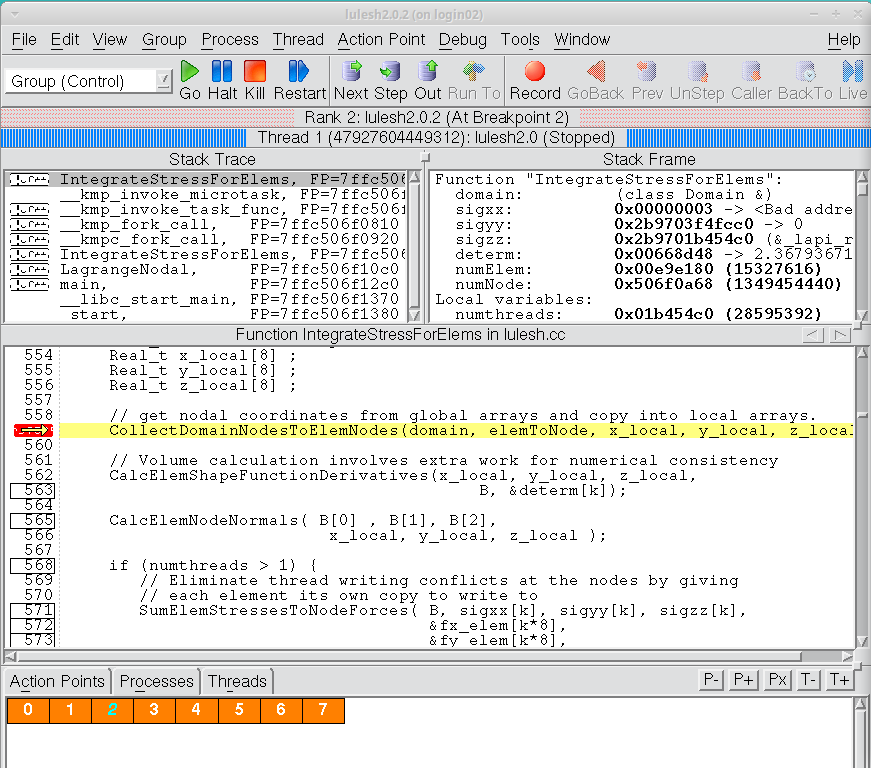
\includegraphics[scale = 0.5]{totalview.png}
\captionof{figure}{Process Window} 
\vspace{10mm}
\hspace{15mm}
\\
\begin{table}
\centering
\begin{tabular}{| p{2cm} | p{10cm} |}
\hline
\textbf{Command name} & \textbf{Description} \\ \hline
Go                   & Starts the execution of the program                   \\ \hline
Halt                  & Pauses the execution of the program. This can be useful if you suspect that the program is stuck in an infinite loop.                \\ \hline
Kill                 & Stops the execution of the program						   \\ \hline
Restart                 & Restarts the execution of the program from the beginning						   \\ \hline
Next                 & Moves to the next step in the current scope (i.e. if a function is called, it is carried out completely and the program stops when it reaches the first step after the function)						   \\ \hline
Step                 & Moves to the next step in the execution. This usually entails stepping into a function and showing the first step within						   \\ \hline
Out                 & Moves to the next step in the parent scope (i.e. if the current step is in a function, the function executes and the program stops when it reaches the first step after the function)						   \\ \hline
Run To                 & When a function is selected, run to allows the program to carry out all steps between its current position and the selected function.					   \\ \hline

\end{tabular} 
\caption{Run controls description}
\end{table}  

\item \textbf{Setting breakpoints}:

Breakpoint is set by clicking on the line number where the break is required or by right clicking on the line and selecting "Set Breakpoint" in the dropdown menu. When the breakpoint has successfully been set a red "STOP" will appear on the line number. When the program is run using the button "Go" it will then carry out all jobs until it reaches this breakpoint, at which point it will pause all jobs allowing the execution to be continued from this point. This can however be problematic as processes rarely run at exactly the same speed. It would therefore be necessary to force each individual thread to then get to this point (without pressing "Go" as this would make the thread that has reached the breakpoint go past it). To help with this, barriers exist. Barriers are points which all threads must reach before any thread continues. They are set by right clicking on the line and selecting "Set Barrier" in the dropdown menu. \\

\item \textbf{Diving into functions}:

Diving into a function opens the source code of that function. This can be done by right clicking on a function and selecting "Dive" in the dropdown menu. During step-by-step execution it can also be done by clicking "Step". This means that all steps carried out by the program can be analysed, including those which are not immediately
visible. \\

\item \textbf{View memory (variables and arrays)}:

A list of variables is shown in the stack frame pane along with some basic information about them. More information can be found by diving into the variables. This can be done by double clicking on them in the stack frame pane. One structure that can be more difficult to visualise is an array. Although we can dive into it as with a structure, it is likely that there will be too many variables to get a clear picture of what the array contains. By clicking "Visualize" in the "Tools" menu of the variable popup-dive window, it is possible to get a view. This allows us to have an idea of the magnitude of the values of the array as well as the uniformity. \\

\end{enumerate}


\item \textbf{Give a short explanation on why these operations are important in a debugger}

\begin{enumerate}
\item \textbf{Control execution}:

Control execution allow the user to progress step by step to
find correctness of program and on which line the results diverge from what is expected. User can dive into important part of the code and the omit the ones which are not so relevant. \\

\item \textbf{Setting breakpoints}:

A user sometimes has an idea where the problem might be. It is therefore not necessary to follow the whole execution step by step but only a certain portion of the execution, value of some variables at particular time etc. A breakpoint is used to help this. \\ \\

\item \textbf{Diving into functions}:

As mentioned in setting breakpoints, when debugging, it is likely that a user has an idea of where the problem may be. It is therefore important to be able to navigate to the correct portion of the code. This is done by diving into functions which in turn facilitates efficient use of resources and time.\\

\item \textbf{View memory (variables and arrays)}:

During the actual debugging process there are indicators which allow user to see when a program begins to act differently to what was expected of the variables. It is therefore important to be able to monitor the variables and erroneous values can be quickly located. \\
\end{enumerate}
\end{enumerate}

\section{MPI with TotalView}

\subsection{Task 4}

\begin{enumerate}
\item \textbf{State the name of the array you decided to visualize and include a snapshot of its visualization in the report. It is not necessary to understand the actual meaning of the values in the array.} 

The array which we decided to visualize is of type domain locDom which is defined in line 2681 of lulesh.cc file. Snapshot of its visualization is as below. \\

\hspace{25mm}
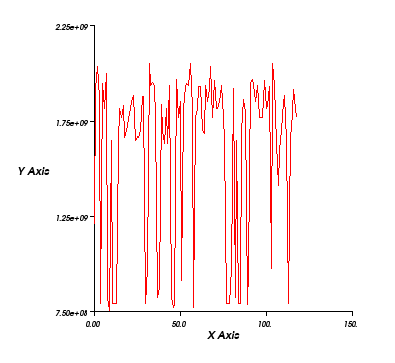
\includegraphics[scale = 0.75]{locdom.png}
\captionof{figure}{Visualization} 
\vspace{5mm}


\item \textbf{What is the name of the MPI rank variable in the benchmark?}

The name of the MPI rank variable in the benchmark is myRank which is declared in 2682 line of lulesh.cc \\

\item \textbf{What is the name of the MPI size variable in the benchmark?}

The name of the MPI size variable in the benchmark is numRanks which is declared in 2681 line of lulesh.cc \\

\item \textbf{Where are these variables first set in the benchmark’s source code (file name and line number)?}

The MPI size variable numRanks is first set in 2702 line of lulesh.cc and is argument to MPI\_Comm\_size function. The number of processes in the group associated with the communicator MPI\_COMM\_WORLD is returned in numRanks when MPI\_Comm\_size is called.\\ MPI rank variable myRank is first set in 2703 line of lulesh.cc and is argument to MPI\_Comm\_rank function. The rank of each process is returned in myRank when MPI\_Comm\_rank is called.\\ \\

\hspace{10mm}
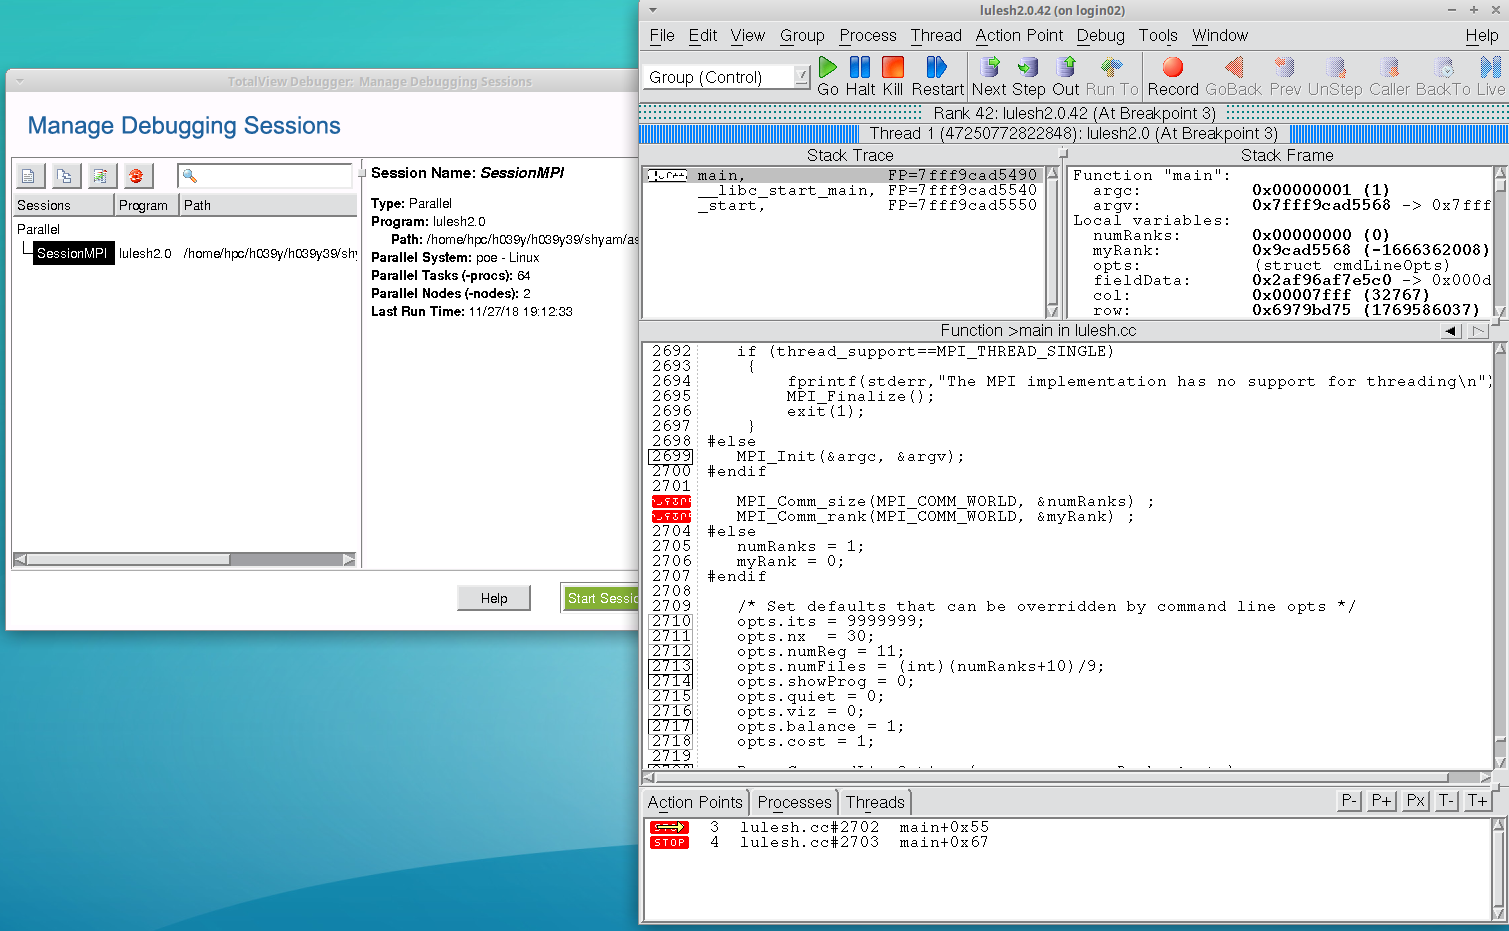
\includegraphics[scale = 0.4]{Totalview3.png}
\captionof{figure}{MPI benchmark breakpoints} 
\vspace{5mm}

\end{enumerate}

\section{MPI+OpenMP with TotalView}

\subsection{Task 5}

\begin{enumerate}
\item \textbf{Justify in the report the core and thread combination used.}

The number of processors should be integer cubed i.e. 1, 8, 27, 64. Also, the product of the number of threads and the number of processes must be less than the number of cores on the node. Since we use 2 nodes and the number of cores in each node is 40, so the total cores available is 80. Hence we can use 8 MPI process and 10 OpenMP threads and thus can populate on all the cores. \\


\item \textbf{Explain how thread and process counts are controlled in TotalView.}

All TotalView commands operate on a set of processes and threads. This set is called a Process/Thread set. While creating a new parallel program session, we can set the thread and process count as shown in below figure. The process counts and number of nodes are set in PARALLEL DETAILS -\textgreater  'Parallel Settings'. The thread count is set in ENVIRONMENT -\textgreater  'Program Environment' . e.g. OMP\_NUM\_THREADS=10 

\hspace{18mm}
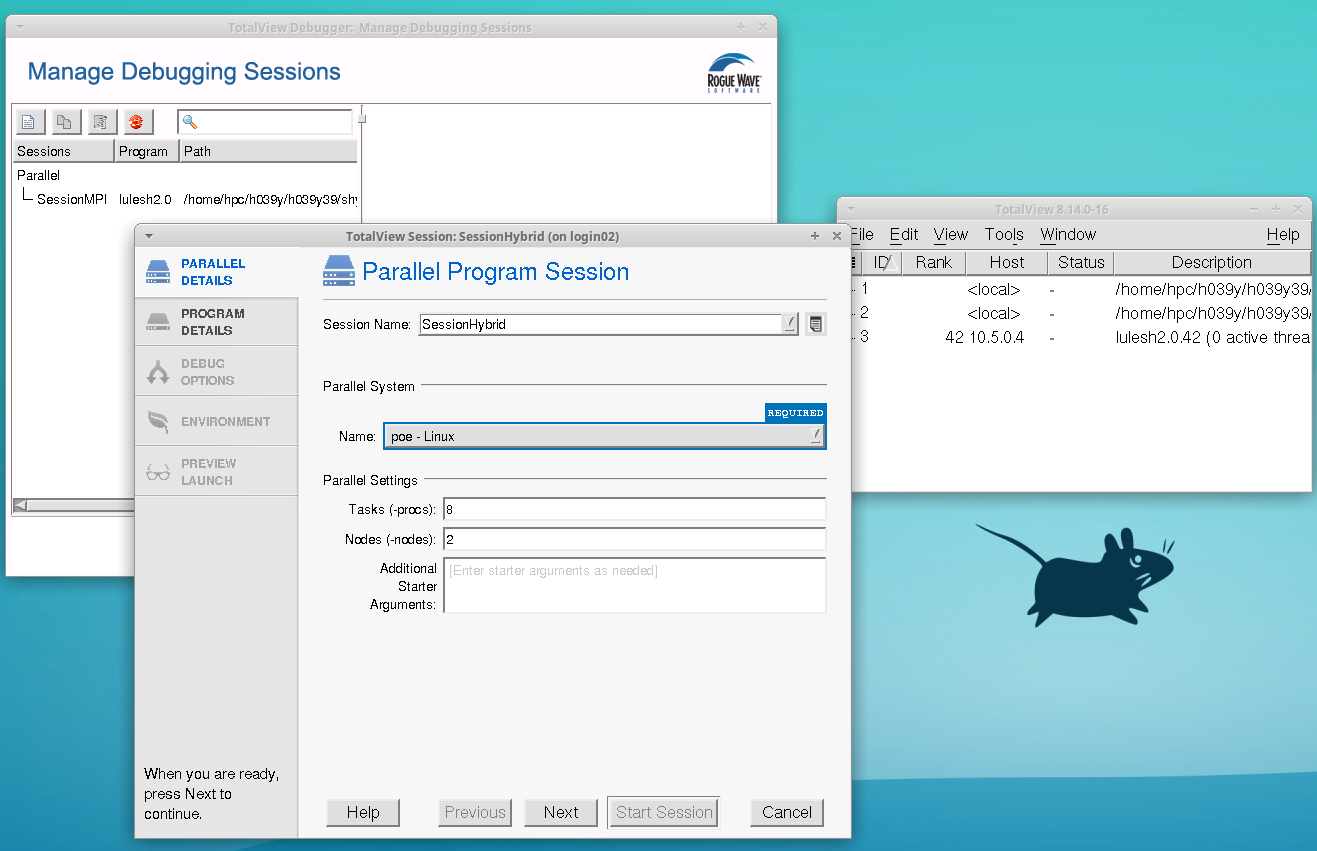
\includegraphics[scale = 0.3]{Hybrid1.png}
\vspace{5mm}

\hspace{25mm}
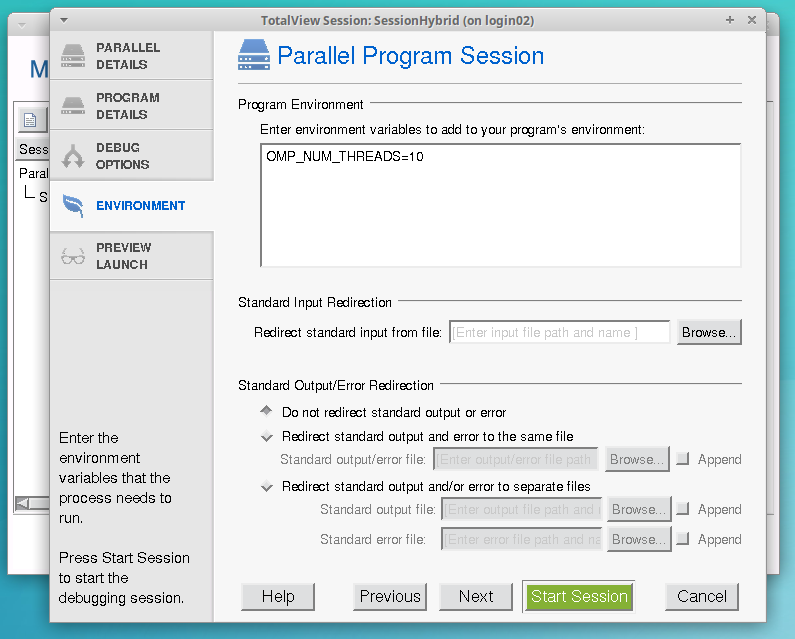
\includegraphics[scale = 0.5]{Hybrid2.png} 
\captionof{figure}{Totalview: MPI + OpenMP} 
\vspace{5mm}


\item \textbf{Explain what the fork-join model is.}

In parallel computing, the fork–join model is a way of setting up and executing parallel programs, such that execution branches off in parallel at designated points in the program, to "join" (merge) at a subsequent point and resume sequential execution. Parallel sections may fork recursively until a certain task granularity is reached. Fork–join can be considered a parallel design pattern. \\

\hspace{3cm}
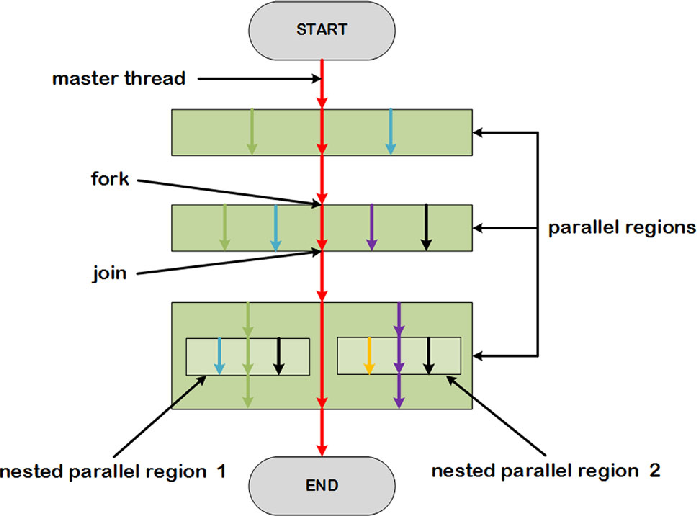
\includegraphics[scale = 1.5]{joinfork.png} 
\captionof{figure}{Fork-join model} 

\item \textbf{Include a screen capture of the before and after effect of the fork-join model by navigating to a parallel region and looking at the Threads Pane in TotalView.}

To see TotalView working, we set breakpoints in places aside from the main function. After a thorough investigation of the lulesh code, we found a particularly interesting place to see the efect of the MPI + OpenMP fork-join model. In order to note the changes, screenshots were captured before forking(line 542), after forking(line 559), and after join(line 590).\\

\hspace{30mm}
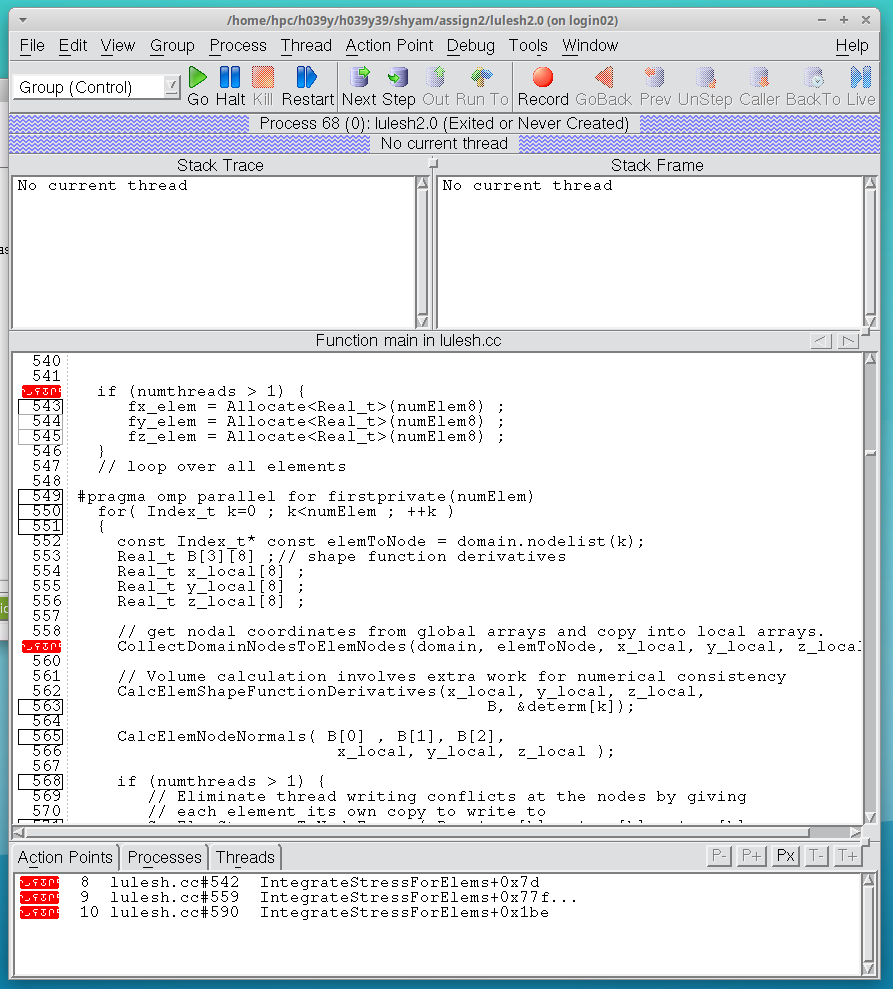
\includegraphics[scale = 0.4]{Hybrid3.png} 
\captionof{figure}{Totalview: MPI + OpenMP Fork-join breakpoints} 
\vspace{20mm}

\hspace{30mm}
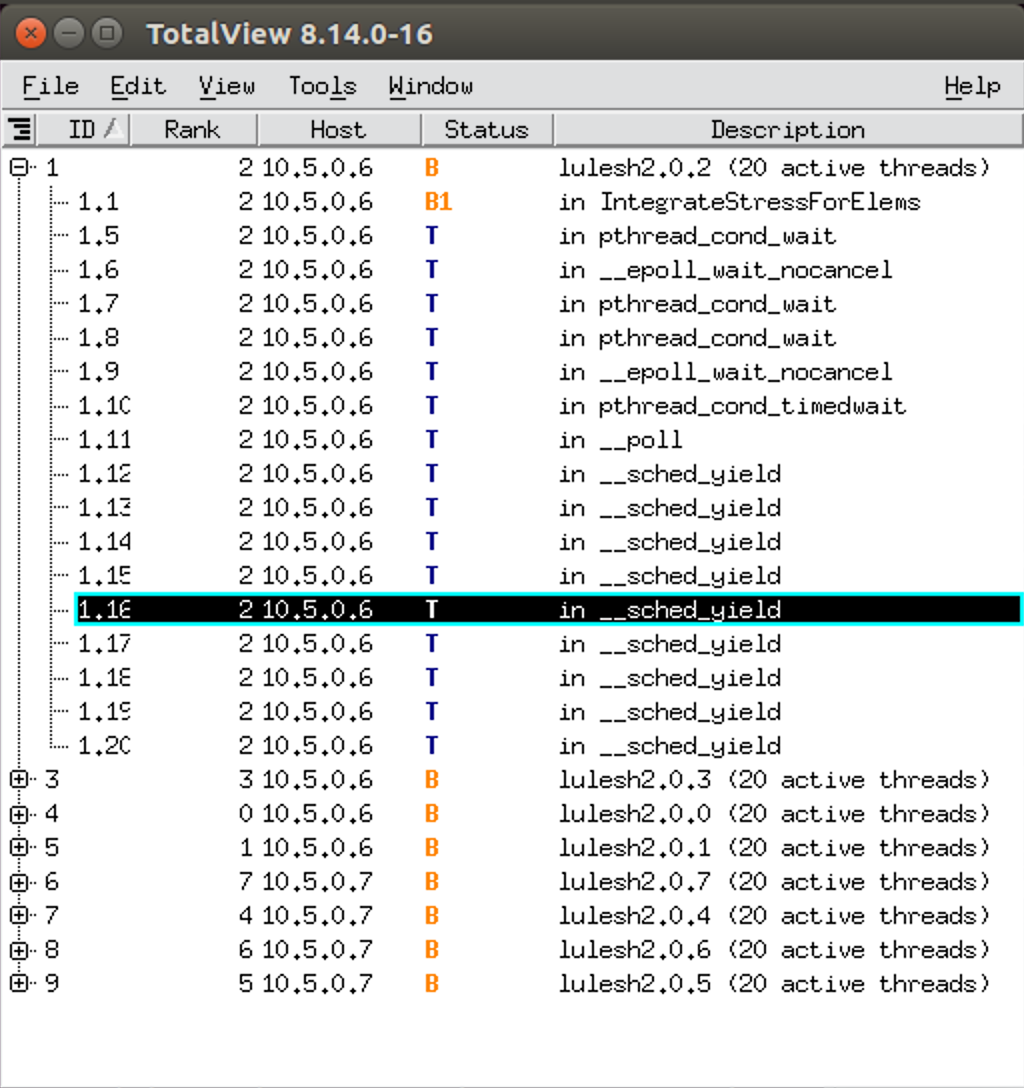
\includegraphics[scale = 0.3]{Hybrid8.png} 
\captionof{figure}{Totalview: MPI + OpenMP Before Fork-Join} 
\vspace{8mm}

\hspace{30mm}
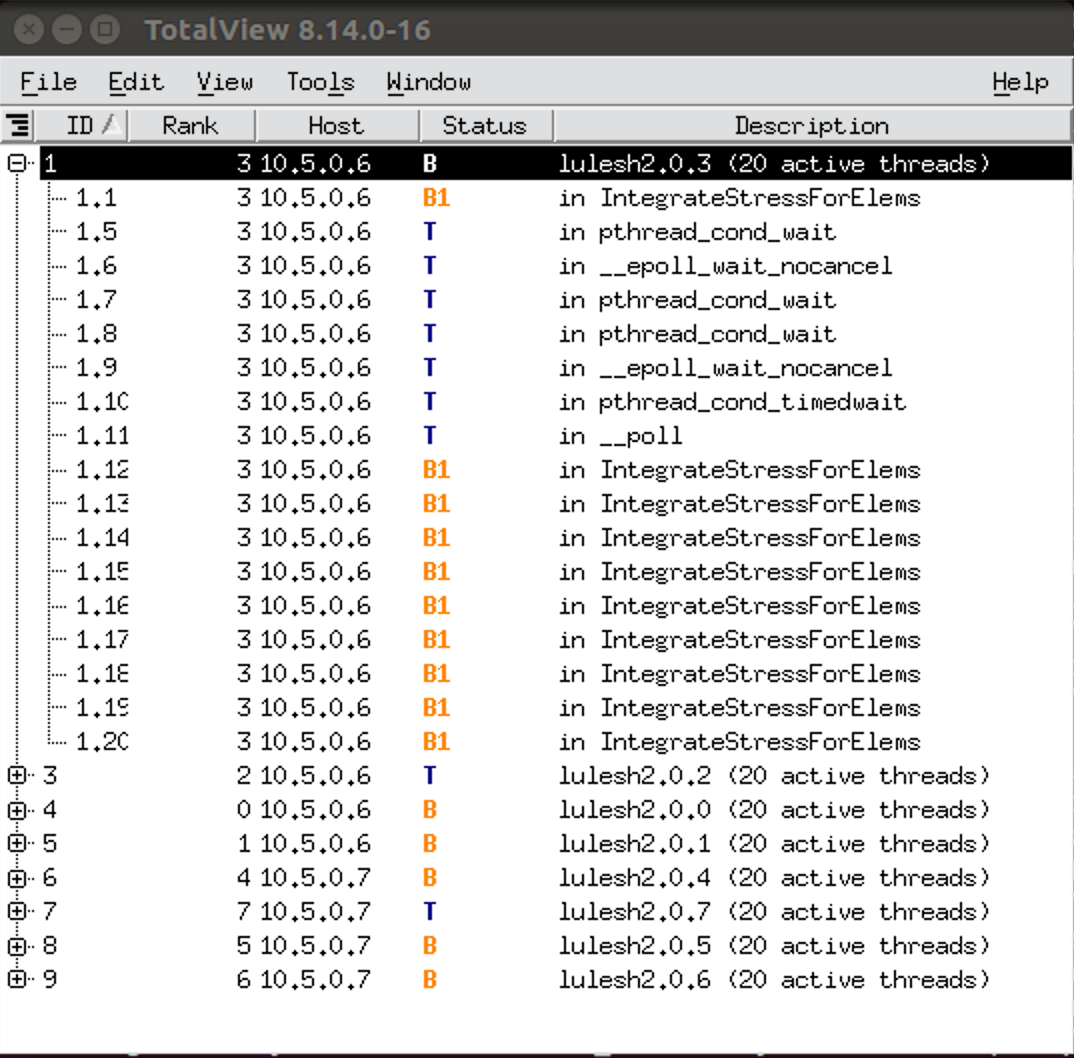
\includegraphics[scale = 0.3]{Hybrid6.png} 
\captionof{figure}{Totalview: MPI + OpenMP During Fork-Join} 
\vspace{8mm}

\hspace{30mm}
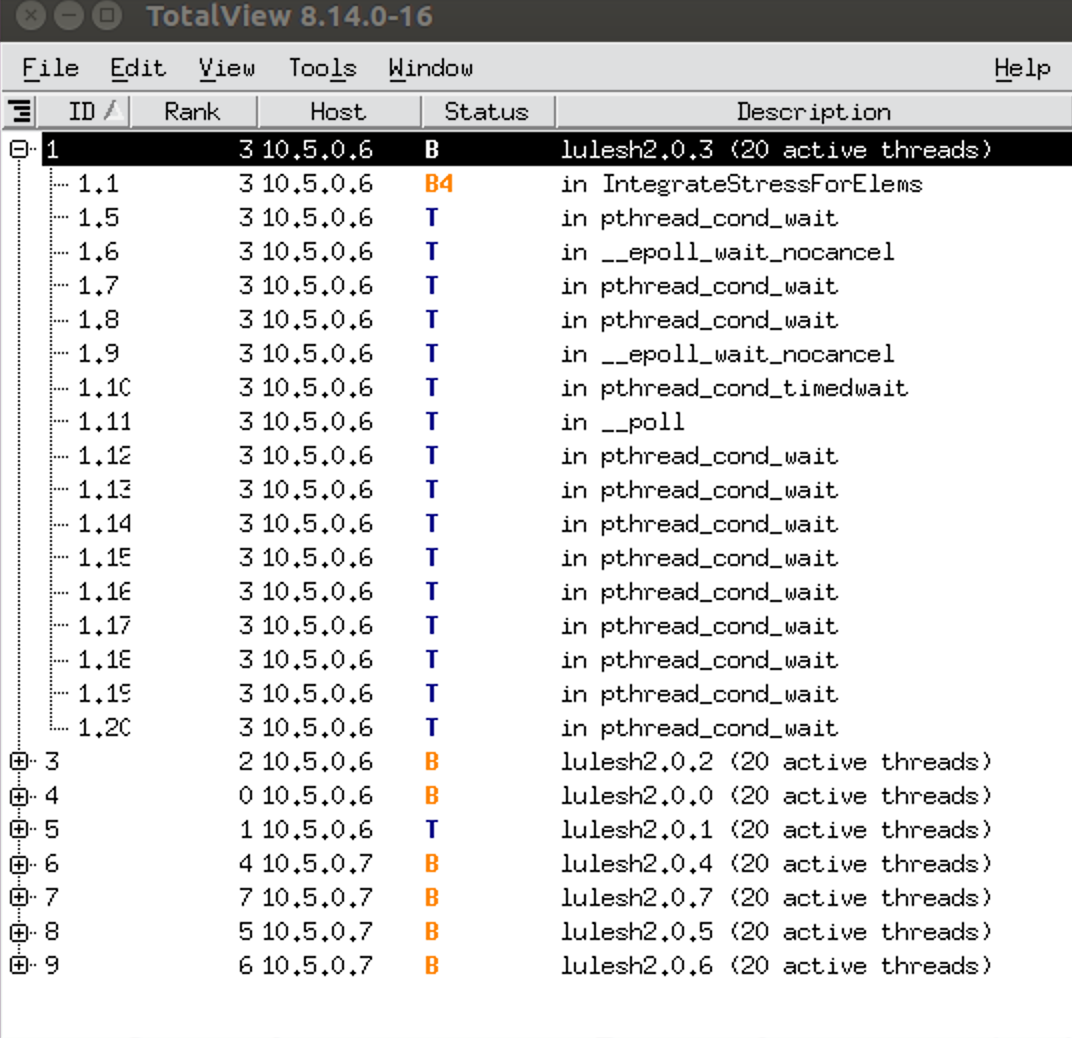
\includegraphics[scale = 0.3]{Hybrid7.png} 
\captionof{figure}{Totalview: MPI + OpenMP After Fork-Join} 
\vspace{8mm}
\end{enumerate}


\section{MPI+OpenMP with Vampir}

\subsection{Task 6}

\begin{enumerate}

\item \textbf{What are the main differences in the way events are recorded by gprof and Score-P?} \\ \\
Gprof is generally used to record events by profiling whereas Score-P is generally used to record events via tracing. \\ \\
Profilers generally operate by sampling ("statistical profiling"). Your program is repeatedly interrupted as it runs, with a fixed interval between interruptions (e.g. every millisecond). The purpose of each interruption is to take a sample, which is done by visiting each running thread, and then examining the stack to discover which functions are running. The effect is similar to stopping execution in a debugger and asking for a backtrace. The profiler records each sample and all of the samples are aggregated into a report or turned into a graph. Tracers do not operate by sampling. Instead, the trace is a log of events within to the program. This log may be detailed enough to report function calls and returns, and execution of other statements. Tracing may require the program to be instrumented, i.e. modified to include code to log events. This instrumentation may be added to the source code or it may be added dynamically to the machine code. Alternatively, tracing may rely on hardware such as the branch trace store \\ \\
A profile cannot be used to reconstruct a trace. This is because the profile omits information about everything that happened between two samples. Many calls and returns may occur between samples: these are invisible in the profile report. In many cases, this missing information is not necessary in order to see where the program is spending most of its time, and it's possible to understand the performance problem without it. A detailed trace may be used to reconstruct a profile. As the trace is a timestamped record of calls and returns, a trace parsing tool can track the state of the stack at each point in time. If the state of the stack is sampled periodically, the result is the same as a profile. \\ \\
Tracing can be useful, but there are additional difficulties when it is used. In many cases a profile will be sufficient for analysing the performance of a program, understanding which parts are slow, and figuring out how to resolve bottlenecks, and these are the problems of interest to most programmers. However, statistical profiles are not suitable for certain problems, such as those in safety-critical systems, and in those cases, tracing may be required.


\item \textbf{Does Vampir support post-mortem or online analysis?}\\ \\
Score-P/Vampir follows post-mortem approach. We need to compile our binaries with Score-P and run the application to generate the trace logs (traces.otf2). All performance data is captured during the application run and written to
the file system for post-mortem analyses. Only after all the events are logged we can open traces.otf2 file with Vampir for visualization.

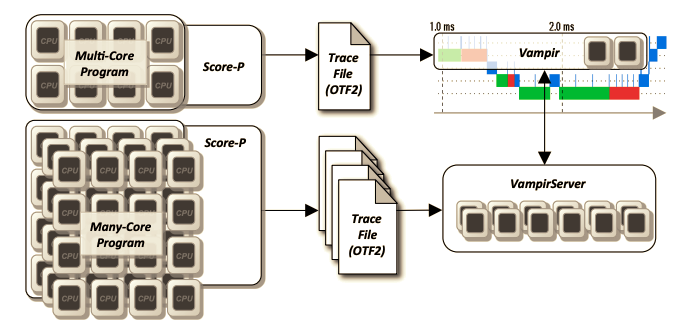
\includegraphics[scale = 0.5]{vampir.png}

\item \textbf{Explain the communication bottlenecks that occur in point-to-point (4 points) and collective MPI communication}
\begin{itemize}
	\item \textbf{Point-to-Point communication bottlenecks}
	\begin{itemize}
		\item Late Sender - If blocking receive is posted before matching send, then the receiving task must wait until the data is sent.\\
		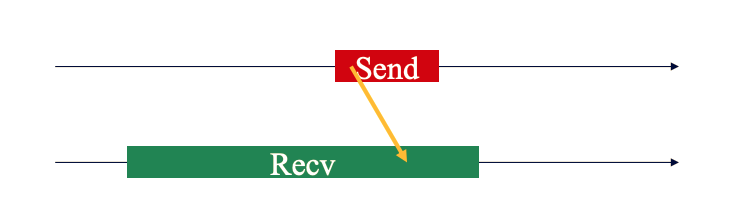
\includegraphics[scale = 0.5]{late_sender.png}
		\item Late Receiver - If send is synchronous and the message is too large, data cannot be sent until receive is posted. Hence the sending task is delayed. \\
		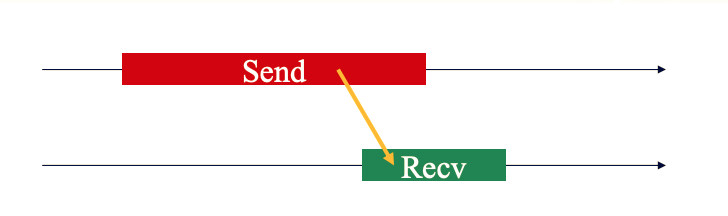
\includegraphics[scale = 0.5]{late_receiver.png}
	\end{itemize}
	\item \textbf{Collective MPI communication bottlenecks}
	\begin{itemize}
		\item Late Broadcaster - If broadcast root is late, all other tasks have to wait. \\
		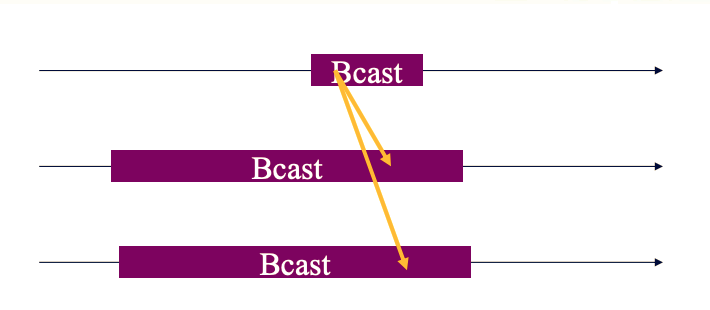
\includegraphics[scale = 0.5]{late_broadcast.png}
		\item Early Reduce - If root task of Reduce is early, it has to wait for all other tasks to enter reduce.\\
		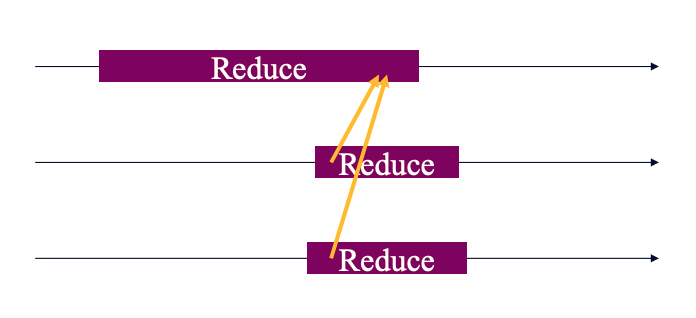
\includegraphics[scale = 0.5]{early_reduce.png}
	\end{itemize}
\end{itemize}



\item \textbf{Take a screen capture of one of the MPI communication bottlenecks from the above question, and describe the situation.} \\ \\
	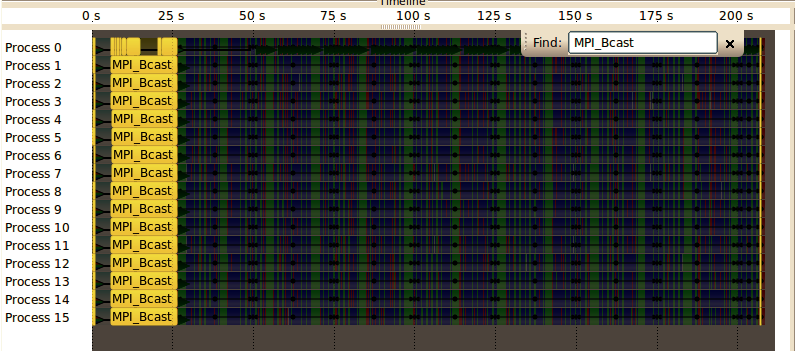
\includegraphics[scale = 0.5]{mpi_bcast.png} \\
A broadcast is one of the standard collective communication techniques. During a broadcast, one process sends the same data to all processes in a communicator. One of the main uses of broadcasting is to send out user input to a parallel program, or send out configuration parameters to all processes. In this example, process zero is the root process, and it has the initial copy of data. All of the other processes receive the copy of data. And as the broadcast root (process 0) is late, all other tasks have to wait to receive the file.

\item \textbf{How does the Performance Radar help in analysis?} \\ \\
The Performance Radar chart displays counter data and provides the possibility to create custom metrics. In contrast to the Counter Data Timeline the Performance Radar shows one counter for all processes at once. The values of counter are shown for all processes and threads at once and are displayed in a color-coded fashion. It also has a number of adjustable options. Thus it is a convenient way to single out certain metric and to visualize how it behaves across different processors and threads over time. For e.g. \textit{Set Chart Mode} allows to define whether minimum, maximum, or average values should be shown. This setting comes into effect when multiple measured data points need to be displayed on one pixel. If Maximum or Minimum is active, the data point with the highest or lowest value is displayed, respectively. In case of Average the average of all data points on the respective pixel width is displayed


\item \textbf{Describe the MPI message pattern in the Communication Matrix tab.} \\ \\
The “Communication Matrix View” is another way of analyzing communication imbalances. It shows information about messages sent between processes. \\ \\
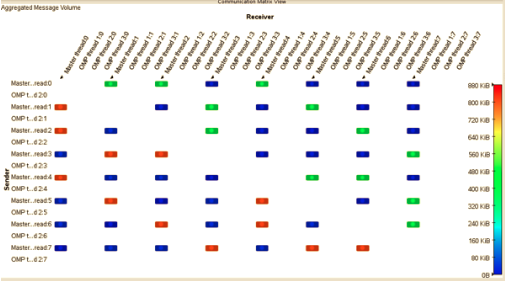
\includegraphics[scale = 0.5]{communication.png} \\ \\
The chart, as shown in the above figure is figured as a table. Its rows represent the sending processes whereas the columns represent the receivers. The color legend on the right indicates the displayed values. It adapts automatically to the currently shown value range. It is possible to change the type of displayed values. Different metrics like the average duration of messages passed from sender to recipient or minimum and maximum bandwidth are offered. 

\item \textbf{Take a screen capture of a fork-join, and describe the situation.} \\ \\
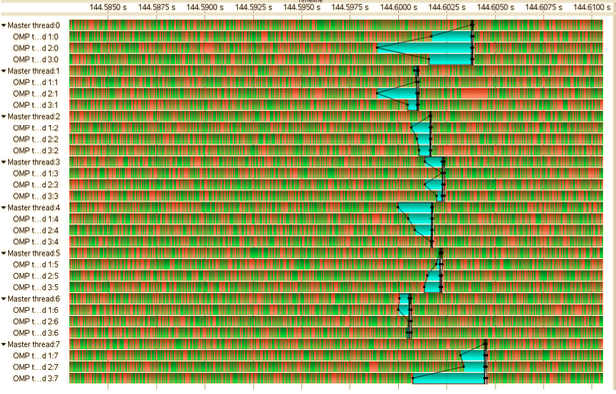
\includegraphics[scale = 0.5]{fork.png} \\ \\
\begin{itemize}
	\item Above region corresponds to parallelized loops inside function void InitStressTermsForElems()
	\item The blue region corresponds to the idle time spend waiting for the threads due to load imbalance
	\item For different processors, the idle regions are of different duration with different start and end time
\end{itemize}


\item \textbf{Do you observe any performance bottlenecks from Section 3.1 (Task 1) in the code?} \\ \\
We observe the following performance bottlenecks from Section 3.1 (Task 1) in the code:
\begin{itemize}
	\item Load Imbalance - In the parallel program load imbalance occurs as one or more thread/process has significantly more to do than the others. This results in threads/processes idling while they wait for the thread with the largest load to complete its work. During this period the program is in effect running in serial and is thus not utilising the benefits of parallel programming.
	\item Parallelization Overhead - Parallel overhead refers to tasks that are not necessary for a serial program. It includes tasks such as starting and terminating threads and synchronising jobs. We see that MPI\_Init and MPI\_Barrier are causing huge parallel overheads at the beginning of the program.
\end{itemize}

\end{enumerate}

\section{Contribution}

\begin{enumerate}
\item \textbf{Smith} \\ 
 Built MPI and MPI+OpenMP binaries. \\
 Performance analysis with Vampir, which involved preparing and running the benchmark for Score-P.\\
 Understanding MPI+OpenMP with Vampir. \\ 

\item \textbf{Shyam} \\ 
 Understanding of the assignment and final report creation.  \\
 Understanding Parallel programming Challenges. \\
 Worked on MPI with TotalView.\\

\item \textbf{Siddhesh} \\ 
 Understanding TotalView GUI and different operations performed in TotalView.  \\
 Worked on MPI + OpenMP with TotalView. \\

\end{enumerate}

\end{titlepage}


\end{document}
